\documentclass{beamer}
\hypersetup{pdfpagemode=FullScreen}
\usetheme{Boadilla}

\usepackage{graphicx}
\usepackage{import}

\title{Path Connected Inverse Limits}
\author{Joseph Camacho}
\institute{Brigham Young University}
\date{February 26, 2021}


\newcommand{\HE}{\mathbb{H}}
\newcommand{\conj}{\bar}
\DeclareMathOperator{\Aut}{Aut}
%\DeclareMathOperator{\ker}{ker}

\begin{document}

\begin{frame}
\titlepage
\end{frame}

\begin{frame}
\frametitle{Overview}
I am looking at when inverse limits of normal covering spaces over the Hawaiian Earring are path connected.  I have been researching for just over a month, so there's still much to explore.

\begin{figure}
\centering
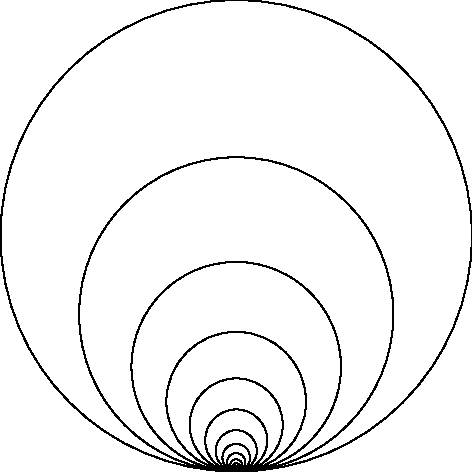
\includegraphics[height=5cm]{images/hawaiian_earring}
\caption{Hawaiian Earring}
\end{figure}
\end{frame}

\begin{frame}
\frametitle{Fundamental Group}
\begin{itemize}
\item  Equivalence classes of loops
\item  Group operation is concatenation end to end
\item  Denoted $\pi_1(X, x_0)$ or $\pi_1(X)$.
\end{itemize}
\begin{figure}[h]
\centering{
\resizebox{!}{6cm}{\fontsize{40}{48}\selectfont \import{images/}{fundamental_group.pdf_tex}}
}
\end{figure}
\end{frame}

\begin{frame}[allowframebreaks]
\frametitle{Covering Space}
A cover $p : E \to X$ is a way of "unrolling" a space $X$.
\begin{figure}[h]
\centering{
\resizebox{8cm}{!}{\fontsize{40}{48}\selectfont \import{images/}{real_line_circle.pdf_tex}}
}
\end{figure}

\pagebreak

Properties:
\begin{itemize}
\item  If $X$ is path connected, so is $E$.
\item  Paths in $X$ starting at $x_0$ have a unique lift starting at $e_0$.
\item  $p_*$ is an inclusion from $\pi_1(E)$ to $\pi_1(X)$.
\end{itemize}
\begin{figure}[h]
\centering{
\resizebox{7cm}{!}{\fontsize{40}{48}\selectfont \import{images/}{covering_space.pdf_tex}}
}
\end{figure}
\end{frame}


\begin{frame}[allowframebreaks]
\frametitle{Inverse Limit}
\begin{itemize}
\item  Way of successively approximating a space
\item  Example:  Hawaiian Earring is the inverse limit of bouquets of circles:
\begin{figure}[h]
\centering{
\resizebox{8cm}{!}{\fontsize{40}{48}\selectfont \import{images/}{inverse_limit.pdf_tex}}
}
\end{figure}

\item  When path connected, the inverse limit of covering spaces behaves much like a covering space.
\end{itemize}

\pagebreak

Inverse limits also exist for groups.
\begin{itemize}
\item  Similar definition to inverse limit for topological spaces
\item  $E = \varprojlim X_n$ does \textbf{not} imply that $\pi_1(E) \cong \varprojlim \pi_1(X_n)$.
\item  Example:  As above, let $X_n$ be the bouquet of $n$ circles.  Then $\varprojlim X_n = \HE$, but $\varprojlim \pi_1(X_n) \ncong \pi_1(\HE)$.
\end{itemize}

\begin{figure}[h]
\centering{
\resizebox{8cm}{!}{\fontsize{40}{48}\selectfont \import{images/}{inverse_limit.pdf_tex}}
}
\end{figure}
\end{frame}


\begin{frame}[allowframebreaks]
\frametitle{Deck Transformation}
\begin{itemize}
\item  An automorphism on $E$ such that $p \circ d = p$.
\item  Forms a group (through composition) $\Aut(E)$.
\end{itemize}
\begin{figure}[h]
\centering{
\resizebox{!}{4cm}{\fontsize{40}{48}\selectfont \import{images/}{deck_transformation_commutative.pdf_tex}}
}
\end{figure}

\pagebreak

A covering space is \textit{normal} if for each point $e$ in the fiber of $x_0$ there is a deck transformation that sends $e_0$ to $e$.
Properties:
\begin{itemize}
\item  All fiber points look alike.
\item  $\pi_1(E, e_0)$ is a normal subgroup of $\pi_1(X, x_0)$.
\item  $\Aut(E)$ is isomorphic to $\pi_1(X) / \pi_1(E)$.
\end{itemize}

\pagebreak

\begin{figure}[h]
\centering{
\resizebox{!}{6cm}{\fontsize{40}{48}\selectfont \import{images/}{deck_transformation.pdf_tex}}
\resizebox{!}{6cm}{\fontsize{40}{48}\selectfont \import{images/}{not_normal_cover.pdf_tex}}
}
\end{figure}
\end{frame}


\begin{frame}
\frametitle{The Main Question}
Let $X_0 = \HE$ be the Hawaiian Earring.  For $n \in \mathbb{Z}_+$, let $p_n : X_n \to X_{n-1}$ be a normal cover.  Furthermore, assume that $X_n$ is a covering space of $\HE$.  When is $\varprojlim X_n$ path connected?
\end{frame}

\begin{frame}
\frametitle{Relation to Fundamental Groups}
\textbf{Lemma}:  Let $\phi : \pi_1(\HE) \to \varprojlim \pi_1(X) / \pi_1(X_n)$ be defined by
$$\phi(g) = (g\pi_1(X_1), g\pi_1(X_2), \dots).$$
Then $\varprojlim X_n$ is path connected if and only if $\phi$ is surjective.

\begin{figure}[h]
\centering{
\resizebox{!}{3cm}{\fontsize{40}{48}\selectfont \import{images/}{phi_lemma.pdf_tex}}
}
\end{figure}
\end{frame}

\begin{frame}[allowframebreaks]
\frametitle{Example 1 (Free Groups)}
For $n = 1, 2, 3, \dots$, let $\alpha_n$ be a loop counterclockwise around the $n$th circle of the Hawaiian Earring.  Let $a_n = [\alpha_n]$.

Let $q^n$ be the function that collapses all but the first $n$ circles.

\begin{figure}[h]
\centering{
\resizebox{!}{3cm}{\fontsize{20}{24}\selectfont \import{images/}{labelled_loops.pdf_tex}}
\resizebox{!}{3cm}{\fontsize{40}{48}\selectfont \import{images/}{collapse_circles.pdf_tex}}
}
\end{figure}

\pagebreak

There exists a covering space $X_n$ with fundamental group $\ker(q_*^n)$.  It looks like the Cayley graph of the free group with $n$ generators.
\begin{figure}[h]
\centering
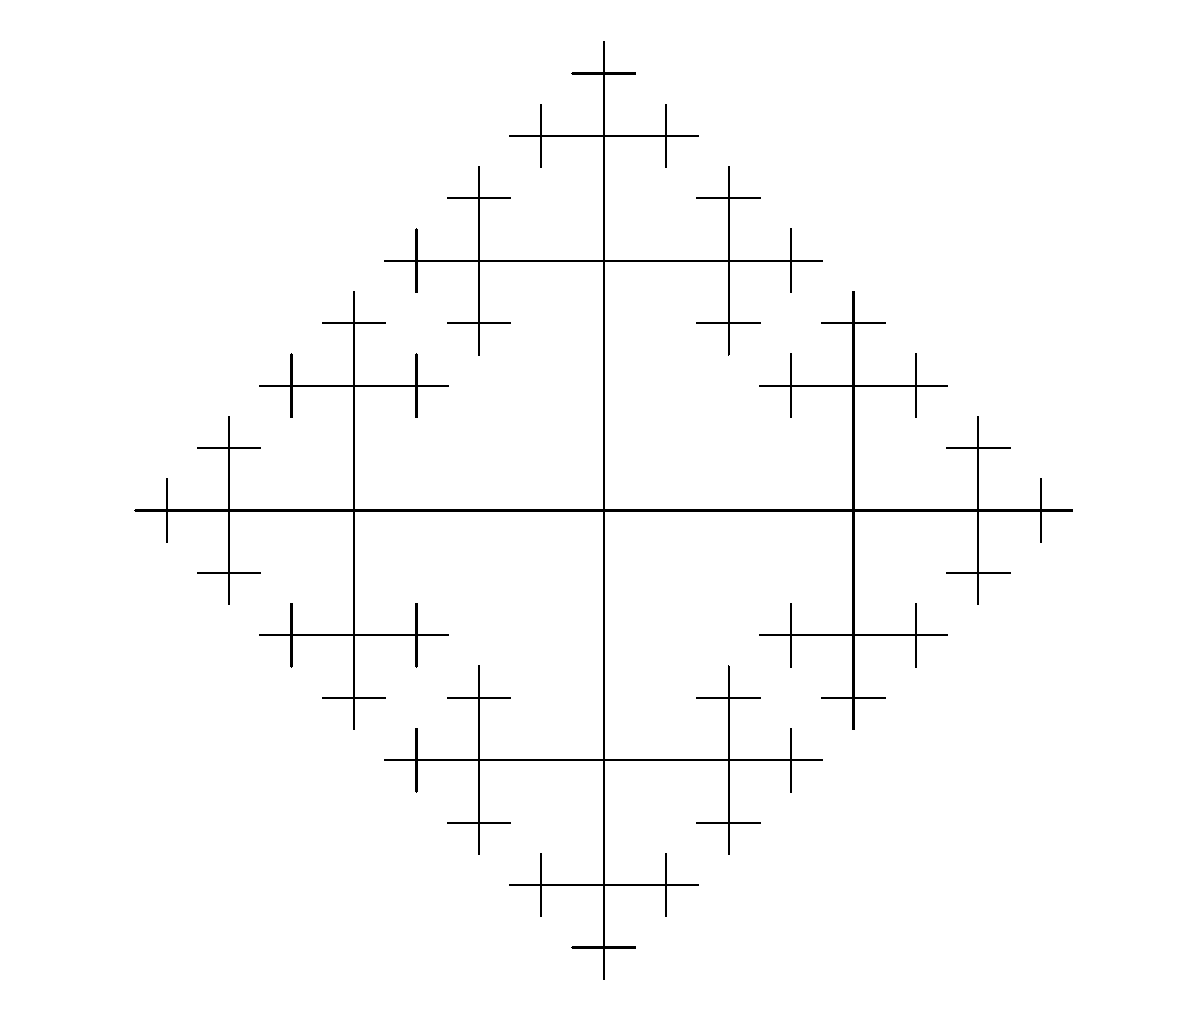
\includegraphics[height=4cm]{images/cayley_graph.pdf}
\caption{$X_2$}
\end{figure}

\pagebreak

$\varprojlim X_n$ is \textbf{not} path connected.  Why?

You can construct coherent sequences that would require going around the first loop infinitely many times.  For instance, the element
$$(1\pi_1(X_1), [a_1, a_2]\pi_1(X_2), [a_1, a_2][a_1, a_3]\pi_1(X_3), \dots) \in \varprojlim \pi_1(\HE) / \pi_1(X_n)$$
is unattainable by $\phi$.

\begin{figure}[h]
\centering
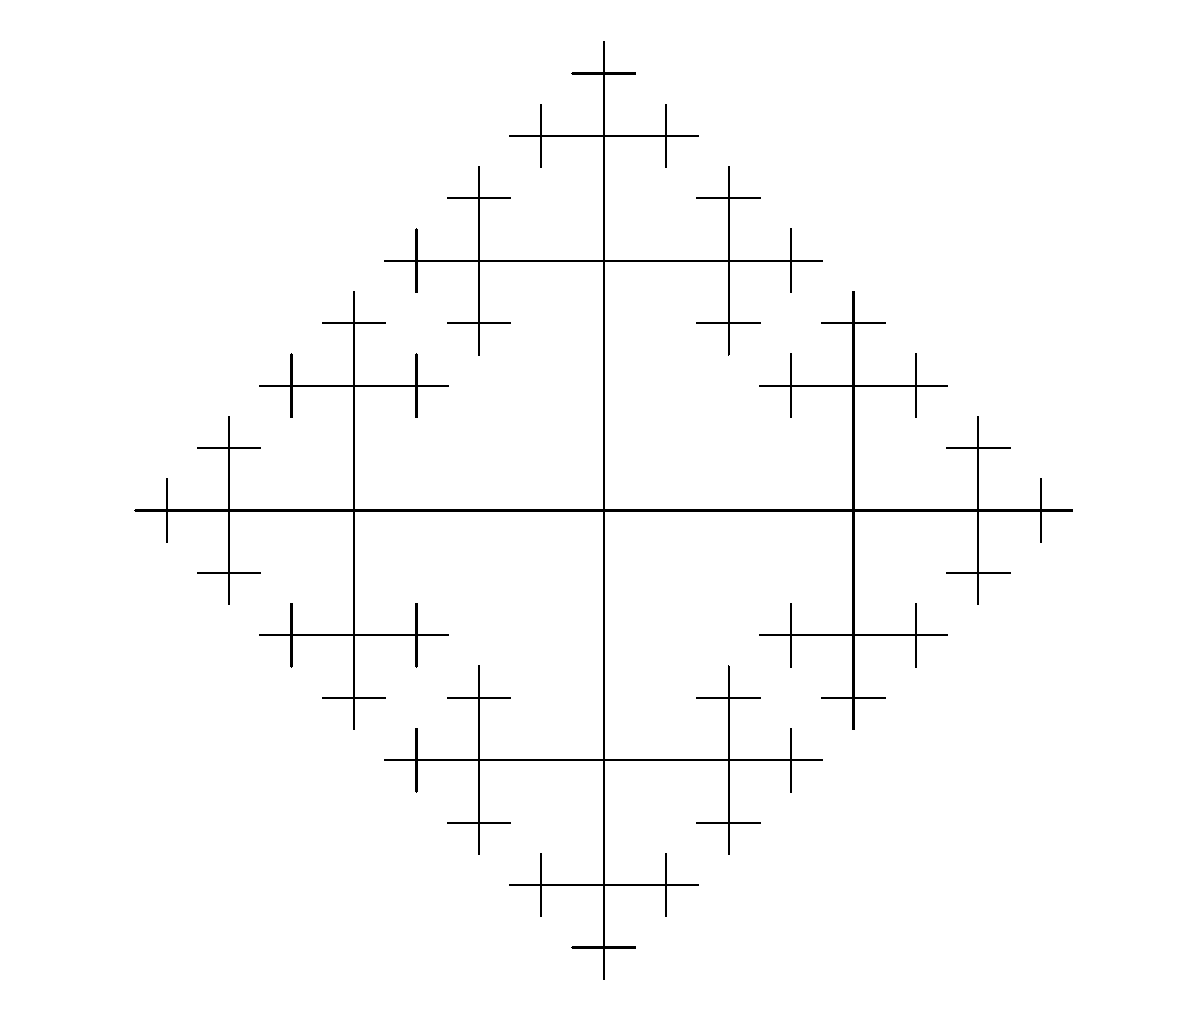
\includegraphics[height=4cm]{images/cayley_graph.pdf}
\end{figure}
\end{frame}


\begin{frame}[allowframebreaks]
\frametitle{Example 2 (Wireframe)}
Define $a_n$ and $q_n$ as in the previous example.
Let
$$K_n = \langle \langle \ker(q_*), [a_i, a_j] : 1 \le i < j \le n \rangle \rangle.$$
There exists a covering space $X_n$ of $\HE$ with fundamental group $K_n$.

The commutator $[a_i, a_j]$ has the effect of joining together the two ends of $a_ia_j$ and $a_ja_i$.  The fundamental group looks like a wireframe:
\begin{figure}[h]
\centering

\includegraphics[height=3cm]{images/wireframe.pdf}
\caption{$X_2$}
\end{figure}

\pagebreak

$\varprojlim X_n$ is path connected.  Why?

Let
$$(w_1 \pi_1(X_1), w_2 \pi_1(X_2), \dots) \in \varprojlim \pi_1(\HE) / \pi_1(X_n).$$
Because all the $a_i$ commute with each other modulo $\pi_1(X_n)$, we can rearrange the $w_n$ into the form
\begin{align*}
w_1 \pi_1(X_1) &= a_1^{k_1} \pi_1(X_1),\\
w_2 \pi_1(X_2) &= a_1^{k_1} a_2^{k_2} \pi_1(X_2),\\
w_3 \pi_1(X_3) &= a_1^{k_1} a_2^{k_2} a_3^{k_3} \pi_1(X_3),\\ 
\dots.
\end{align*}

Let $g$ be a path that in the interval $[2^{-n}, 2^{-n + 1}]$ wraps around the $i$th loop $k_i$ times.  Under $\phi$ this path maps to the desired element.

\end{frame}


\begin{frame}
\frametitle{Summary}
These examples show that some sense of commutativity is required in order for the inverse limit to be path connected.  My research aims to discover exactly when that is.  Right now, I conjecture that $\varprojlim X_n$ is path connected if and only if
$$[a_i, a_j] \pi_1(X_n) \in \ker(q_*^i) \pi_1(X_n)$$
for all integers $i < j$ and $n$.
\end{frame}


\end{document}